\section{peo\-Sync\-Multi\-Start$<$ EOT $>$ Class Template Reference}
\label{classpeo_sync_multi_start}\index{peoSyncMultiStart@{peoSyncMultiStart}}
The {\bf peo\-Sync\-Multi\-Start}{\rm (p.\,\pageref{classpeo_sync_multi_start})} class provides the basis for implementing the synchronous multi-start model, for launching several solution-based algorithms in parallel on a specified initial population.  


{\tt \#include $<$peo\-Sync\-Multi\-Start.h$>$}

Inheritance diagram for peo\-Sync\-Multi\-Start$<$ EOT $>$::\begin{figure}[H]
\begin{center}
\leavevmode
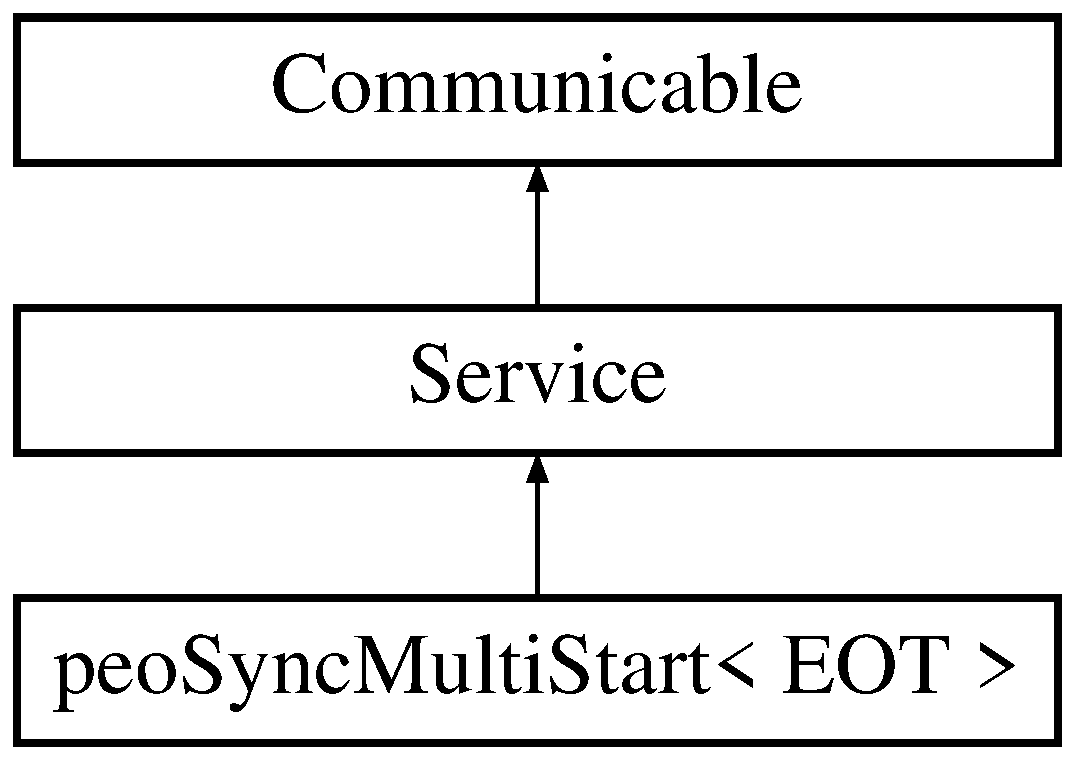
\includegraphics[height=3cm]{classpeo_sync_multi_start}
\end{center}
\end{figure}
\subsection*{Public Member Functions}
\begin{CompactItemize}
\item 
{\bf peo\-Sync\-Multi\-Start} (eo\-Continue$<$ EOT $>$ \&\_\-\_\-cont, eo\-Select$<$ EOT $>$ \&\_\-\_\-select, eo\-Replacement$<$ EOT $>$ \&\_\-\_\-replace, mo\-Algo$<$ EOT $>$ \&\_\-\_\-ls, eo\-Pop$<$ EOT $>$ \&\_\-\_\-pop)
\begin{CompactList}\small\item\em Constructor function - several simple parameters are required for defining the characteristics of the multi-start model. \item\end{CompactList}\item 
void {\bf operator()} ()
\begin{CompactList}\small\item\em Operator which synchronously executes the specified algorithm on the individuals selected from the initial population. \item\end{CompactList}\item 
void {\bf pack\-Data} ()
\begin{CompactList}\small\item\em Auxiliary function for transferring data between the process requesting the synchronous execution of the specified algorithm and the process which actually executes the algorithm. \item\end{CompactList}\item 
void {\bf unpack\-Data} ()
\begin{CompactList}\small\item\em Auxiliary function for transferring data between the process requesting the synchronous execution of the specified algorithm and the process which actually executes the algorithm. \item\end{CompactList}\item 
void {\bf execute} ()
\begin{CompactList}\small\item\em Auxiliary function for actually executing the specified algorithm on one assigned individual. \item\end{CompactList}\item 
void {\bf pack\-Result} ()
\begin{CompactList}\small\item\em Auxiliary function for transferring data between the process requesting the synchronous execution of the specified algorithm and the process which actually executes the algorithm. \item\end{CompactList}\item 
void {\bf unpack\-Result} ()
\begin{CompactList}\small\item\em Auxiliary function for transferring data between the process requesting the synchronous execution of the specified algorithm and the process which actually executes the algorithm. \item\end{CompactList}\item 
void {\bf notify\-Sending\-Data} ()
\begin{CompactList}\small\item\em Auxiliary function for notifications between the process requesting the synchronous multi-start execution and the processes that performs the actual execution phase. \item\end{CompactList}\item 
void {\bf notify\-Sending\-All\-Resource\-Requests} ()
\begin{CompactList}\small\item\em Auxiliary function for notifications between the process requesting the synchronous multi-start execution and the processes that performs the actual execution phase. \item\end{CompactList}\end{CompactItemize}
\subsection*{Private Attributes}
\begin{CompactItemize}
\item 
eo\-Continue$<$ EOT $>$ \& {\bf cont}\label{classpeo_sync_multi_start_43f4fa9b125baef6fc8b968dfd16f437}

\item 
eo\-Select$<$ EOT $>$ \& {\bf select}\label{classpeo_sync_multi_start_8fc9a3d046023ddd077defec3c23ab3b}

\item 
eo\-Replacement$<$ EOT $>$ \& {\bf replace}\label{classpeo_sync_multi_start_a375ccea98e9bf2a0854dac27df4522f}

\item 
mo\-Algo$<$ EOT $>$ \& {\bf ls}\label{classpeo_sync_multi_start_4d317966de767dcc87eee0286ea7f95d}

\item 
eo\-Pop$<$ EOT $>$ \& {\bf pop}\label{classpeo_sync_multi_start_391178bd6b8a97a08ab4e345f070e967}

\item 
eo\-Pop$<$ EOT $>$ {\bf sel}\label{classpeo_sync_multi_start_dbcc1a069ec72ecd8d40c392640d84b3}

\item 
eo\-Pop$<$ EOT $>$ {\bf impr\_\-sel}\label{classpeo_sync_multi_start_ca10f6d258105e3c4f0d1660db5b7679}

\item 
EOT {\bf sol}\label{classpeo_sync_multi_start_2c2ebe46470d1425f0409897deab435b}

\item 
unsigned {\bf idx}\label{classpeo_sync_multi_start_64191ef79b7b589964ac9c3e23ae6718}

\item 
unsigned {\bf num\_\-term}\label{classpeo_sync_multi_start_773eb9097550d9444f25ca8f48997a30}

\end{CompactItemize}


\subsection{Detailed Description}
\subsubsection*{template$<$class EOT$>$ class peo\-Sync\-Multi\-Start$<$ EOT $>$}

The {\bf peo\-Sync\-Multi\-Start}{\rm (p.\,\pageref{classpeo_sync_multi_start})} class provides the basis for implementing the synchronous multi-start model, for launching several solution-based algorithms in parallel on a specified initial population. 

As a simple example, several hill climbing algorithms may be synchronously launched on the specified population, each algorithm acting upon one individual only, the final result being integrated back in the population. A {\bf peo\-Sync\-Multi\-Start}{\rm (p.\,\pageref{classpeo_sync_multi_start})} object can be specified as checkpoint object for a classic Paradis\-EO evolutionary algorithm thus allowing for simple hybridization schemes which combine the evolutionary approach with a local search approach, for example, executed at the end of each generation. 



Definition at line 51 of file peo\-Sync\-Multi\-Start.h.

\subsection{Constructor \& Destructor Documentation}
\index{peoSyncMultiStart@{peo\-Sync\-Multi\-Start}!peoSyncMultiStart@{peoSyncMultiStart}}
\index{peoSyncMultiStart@{peoSyncMultiStart}!peoSyncMultiStart@{peo\-Sync\-Multi\-Start}}
\subsubsection{\setlength{\rightskip}{0pt plus 5cm}template$<$class EOT$>$ {\bf peo\-Sync\-Multi\-Start}$<$ EOT $>$::{\bf peo\-Sync\-Multi\-Start} (eo\-Continue$<$ EOT $>$ \& {\em \_\-\_\-cont}, eo\-Select$<$ EOT $>$ \& {\em \_\-\_\-select}, eo\-Replacement$<$ EOT $>$ \& {\em \_\-\_\-replace}, mo\-Algo$<$ EOT $>$ \& {\em \_\-\_\-ls}, eo\-Pop$<$ EOT $>$ \& {\em \_\-\_\-pop})}\label{classpeo_sync_multi_start_d29f94aad3c1f443bfffc8b6aee0704c}


Constructor function - several simple parameters are required for defining the characteristics of the multi-start model. 

\begin{Desc}
\item[Parameters:]
\begin{description}
\item[{\em eo\-Continue$<$}]EOT $>$\& \_\-\_\-cont - defined for including further functionality - no semantics associated at this time; \item[{\em eo\-Select$<$}]EOT $>$\& \_\-\_\-select - selection strategy for obtaining a subset of the initial population on which to apply the specified algorithm; \item[{\em eo\-Replacement$<$}]EOT $>$\& \_\-\_\-replace - replacement strategy for integrating the resulting individuals in the initial population; \item[{\em mo\-Algo$<$}]EOT $>$\& \_\-\_\-ls - algorithm to be applied on each of the selected individuals - a {\bf mo\-Algo$<$ EOT $>$}-derived object must be specified; \item[{\em eo\-Pop$<$}]EOT $>$\& \_\-\_\-pop - the initial population from which the individuals are selected for applying the specified algorithm. \end{description}
\end{Desc}


Definition at line 121 of file peo\-Sync\-Multi\-Start.h.

\subsection{Member Function Documentation}
\index{peoSyncMultiStart@{peo\-Sync\-Multi\-Start}!operator()@{operator()}}
\index{operator()@{operator()}!peoSyncMultiStart@{peo\-Sync\-Multi\-Start}}
\subsubsection{\setlength{\rightskip}{0pt plus 5cm}template$<$class EOT$>$ void {\bf peo\-Sync\-Multi\-Start}$<$ EOT $>$::operator() ()}\label{classpeo_sync_multi_start_76385b33fe514f91cb83f0fbecbeb3c2}


Operator which synchronously executes the specified algorithm on the individuals selected from the initial population. 

There is no need to explicitly call the operator - automatically called as checkpoint operator. 

Definition at line 176 of file peo\-Sync\-Multi\-Start.h.

References peo\-Sync\-Multi\-Start$<$ EOT $>$::idx, peo\-Sync\-Multi\-Start$<$ EOT $>$::impr\_\-sel, peo\-Sync\-Multi\-Start$<$ EOT $>$::num\_\-term, peo\-Sync\-Multi\-Start$<$ EOT $>$::pop, Service::request\-Resource\-Request(), peo\-Sync\-Multi\-Start$<$ EOT $>$::sel, peo\-Sync\-Multi\-Start$<$ EOT $>$::select, and Communicable::stop().\index{peoSyncMultiStart@{peo\-Sync\-Multi\-Start}!packData@{packData}}
\index{packData@{packData}!peoSyncMultiStart@{peo\-Sync\-Multi\-Start}}
\subsubsection{\setlength{\rightskip}{0pt plus 5cm}template$<$class EOT$>$ void {\bf peo\-Sync\-Multi\-Start}$<$ EOT $>$::pack\-Data ()\hspace{0.3cm}{\tt  [virtual]}}\label{classpeo_sync_multi_start_8becfab1922b64708dca5a53e2932a5a}


Auxiliary function for transferring data between the process requesting the synchronous execution of the specified algorithm and the process which actually executes the algorithm. 

There is no need to explicitly call the function. 

Reimplemented from {\bf Service} {\rm (p.\,\pageref{class_service_aea4b8f7f8fb88e83862ee4bfd9ab207})}.

Definition at line 135 of file peo\-Sync\-Multi\-Start.h.

References peo\-Sync\-Multi\-Start$<$ EOT $>$::idx, and peo\-Sync\-Multi\-Start$<$ EOT $>$::sel.\index{peoSyncMultiStart@{peo\-Sync\-Multi\-Start}!unpackData@{unpackData}}
\index{unpackData@{unpackData}!peoSyncMultiStart@{peo\-Sync\-Multi\-Start}}
\subsubsection{\setlength{\rightskip}{0pt plus 5cm}template$<$class EOT$>$ void {\bf peo\-Sync\-Multi\-Start}$<$ EOT $>$::unpack\-Data ()\hspace{0.3cm}{\tt  [virtual]}}\label{classpeo_sync_multi_start_2903a441b77cded266b5fb651e17a5b5}


Auxiliary function for transferring data between the process requesting the synchronous execution of the specified algorithm and the process which actually executes the algorithm. 

There is no need to explicitly call the function. 

Reimplemented from {\bf Service} {\rm (p.\,\pageref{class_service_3bd87b444710813d30fd754d4d0b4df3})}.

Definition at line 141 of file peo\-Sync\-Multi\-Start.h.

References peo\-Sync\-Multi\-Start$<$ EOT $>$::sol.\index{peoSyncMultiStart@{peo\-Sync\-Multi\-Start}!execute@{execute}}
\index{execute@{execute}!peoSyncMultiStart@{peo\-Sync\-Multi\-Start}}
\subsubsection{\setlength{\rightskip}{0pt plus 5cm}template$<$class EOT$>$ void {\bf peo\-Sync\-Multi\-Start}$<$ EOT $>$::execute ()\hspace{0.3cm}{\tt  [virtual]}}\label{classpeo_sync_multi_start_a4d1c2943c290de540800087b54dc49b}


Auxiliary function for actually executing the specified algorithm on one assigned individual. 

There is no need to explicitly call the function. 

Reimplemented from {\bf Service} {\rm (p.\,\pageref{class_service_e4f2894e6121e60f38d41cfbd7447ae4})}.

Definition at line 147 of file peo\-Sync\-Multi\-Start.h.

References peo\-Sync\-Multi\-Start$<$ EOT $>$::ls, and peo\-Sync\-Multi\-Start$<$ EOT $>$::sol.\index{peoSyncMultiStart@{peo\-Sync\-Multi\-Start}!packResult@{packResult}}
\index{packResult@{packResult}!peoSyncMultiStart@{peo\-Sync\-Multi\-Start}}
\subsubsection{\setlength{\rightskip}{0pt plus 5cm}template$<$class EOT$>$ void {\bf peo\-Sync\-Multi\-Start}$<$ EOT $>$::pack\-Result ()\hspace{0.3cm}{\tt  [virtual]}}\label{classpeo_sync_multi_start_6c48eb0dae741cff7203b65e226f9616}


Auxiliary function for transferring data between the process requesting the synchronous execution of the specified algorithm and the process which actually executes the algorithm. 

There is no need to explicitly call the function. 

Reimplemented from {\bf Service} {\rm (p.\,\pageref{class_service_e5e4f90b2315e15c2a2913bd370f4cf5})}.

Definition at line 153 of file peo\-Sync\-Multi\-Start.h.

References peo\-Sync\-Multi\-Start$<$ EOT $>$::sol.\index{peoSyncMultiStart@{peo\-Sync\-Multi\-Start}!unpackResult@{unpackResult}}
\index{unpackResult@{unpackResult}!peoSyncMultiStart@{peo\-Sync\-Multi\-Start}}
\subsubsection{\setlength{\rightskip}{0pt plus 5cm}template$<$class EOT$>$ void {\bf peo\-Sync\-Multi\-Start}$<$ EOT $>$::unpack\-Result ()\hspace{0.3cm}{\tt  [virtual]}}\label{classpeo_sync_multi_start_c3cbd1f10a89d1915c5ccf82a2c34a1d}


Auxiliary function for transferring data between the process requesting the synchronous execution of the specified algorithm and the process which actually executes the algorithm. 

There is no need to explicitly call the function. 

Reimplemented from {\bf Service} {\rm (p.\,\pageref{class_service_45c06344edbfa482b91f68e2035a6099})}.

Definition at line 159 of file peo\-Sync\-Multi\-Start.h.

References Service::get\-Owner(), peo\-Sync\-Multi\-Start$<$ EOT $>$::impr\_\-sel, peo\-Sync\-Multi\-Start$<$ EOT $>$::num\_\-term, peo\-Sync\-Multi\-Start$<$ EOT $>$::pop, peo\-Sync\-Multi\-Start$<$ EOT $>$::replace, Communicable::resume(), peo\-Sync\-Multi\-Start$<$ EOT $>$::sel, Thread::set\-Active(), and peo\-Sync\-Multi\-Start$<$ EOT $>$::sol.\index{peoSyncMultiStart@{peo\-Sync\-Multi\-Start}!notifySendingData@{notifySendingData}}
\index{notifySendingData@{notifySendingData}!peoSyncMultiStart@{peo\-Sync\-Multi\-Start}}
\subsubsection{\setlength{\rightskip}{0pt plus 5cm}template$<$class EOT$>$ void {\bf peo\-Sync\-Multi\-Start}$<$ EOT $>$::notify\-Sending\-Data ()\hspace{0.3cm}{\tt  [virtual]}}\label{classpeo_sync_multi_start_32ec0d01d3fd8a9932abd68f4781fc94}


Auxiliary function for notifications between the process requesting the synchronous multi-start execution and the processes that performs the actual execution phase. 

There is no need to explicitly call the function. 

Reimplemented from {\bf Service} {\rm (p.\,\pageref{class_service_81ad4d6ebb50045b8977e2ab74826f30})}.

Definition at line 187 of file peo\-Sync\-Multi\-Start.h.\index{peoSyncMultiStart@{peo\-Sync\-Multi\-Start}!notifySendingAllResourceRequests@{notifySendingAllResourceRequests}}
\index{notifySendingAllResourceRequests@{notifySendingAllResourceRequests}!peoSyncMultiStart@{peo\-Sync\-Multi\-Start}}
\subsubsection{\setlength{\rightskip}{0pt plus 5cm}template$<$class EOT$>$ void {\bf peo\-Sync\-Multi\-Start}$<$ EOT $>$::notify\-Sending\-All\-Resource\-Requests ()\hspace{0.3cm}{\tt  [virtual]}}\label{classpeo_sync_multi_start_fc90282cc4e93cdea8f82fd52dd78fb0}


Auxiliary function for notifications between the process requesting the synchronous multi-start execution and the processes that performs the actual execution phase. 

There is no need to explicitly call the function. 

Reimplemented from {\bf Service} {\rm (p.\,\pageref{class_service_f94cc8a5c2665d4574041737e61e9ffc})}.

Definition at line 192 of file peo\-Sync\-Multi\-Start.h.

References Service::get\-Owner(), and Thread::set\-Passive().

The documentation for this class was generated from the following file:\begin{CompactItemize}
\item 
peo\-Sync\-Multi\-Start.h\end{CompactItemize}
